\documentclass{standalone}
\usepackage{tikz}
\usetikzlibrary{
  calc,
  matrix,
  decorations.pathreplacing,
  arrows,
  shapes.geometric
}
\definecolor{reddish}{RGB}{231,76,60}

\begin{document}
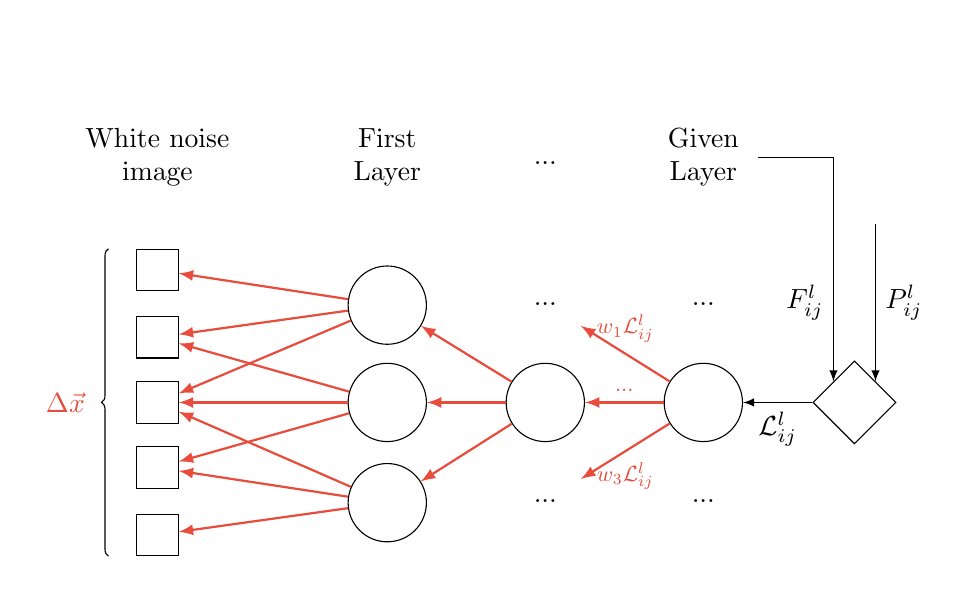
\begin{tikzpicture}[
  plain/.style={
    draw=none,
    fill=none
  },
  dots/.style={
    draw=none,
    fill=none,
    minimum width=3em,
    inner sep=0pt
  },
  input/.style={
    draw,
    rectangle,
    fill=none,
    minimum width=1.5em,
    minimum height=1.5em,
    inner sep=0pt,
  },
  loss/.style={
    draw,
    diamond,
    fill=none,
    minimum width=3em,
    minimum height=3em,
    inner sep=0pt,
  },
  error/.style={
    draw=none,
    fill=reddish
  },
  net/.style={
    matrix of nodes,
    nodes={
      draw,
      circle,
      inner sep=10pt
    },
    nodes in empty cells,
    column sep=0.2cm,
    row sep=-17pt
  },
  >=latex
]

\matrix[net] (mat) {
  % Text row
  |[plain]| \parbox{2cm}{\centering White noise\\image} &
  |[plain]| \parbox{1.2cm}{\centering First\\Layer} &
  |[plain]| ... &
  |[plain]| \parbox{1.2cm}{\centering Given\\Layer} &
  |[plain]| \\
  % Nodes
  |[input]| & |[plain]| & |[plain]|    & |[plain]|    & |[plain]|\\
  |[plain]| &           & |[dots]| ... & |[dots]| ... & |[plain]|\\
  |[input]| & |[plain]| & |[plain]|    & |[plain]|    & |[plain]|\\
  |[plain]| & |[plain]| & |[plain]|    & |[plain]|    & |[plain]|\\
  |[input]| &           &              &              & |[loss]|\\
  |[plain]| & |[plain]| & |[plain]|    & |[plain]|    & |[plain]|\\
  |[input]| & |[plain]| & |[plain]|    & |[plain]|    & |[plain]|\\
  |[plain]| &           & |[dots]| ... & |[dots]| ... & |[plain]|\\
  |[input]| & |[plain]| & |[plain]|    & |[plain]|    & |[plain]|\\
};

% Arrows 1
\draw[<-,reddish,thick] (mat-2-1) to (mat-3-2);
\draw[<-,reddish,thick] (mat-4-1) to (mat-3-2);
\draw[<-,reddish,thick] (mat-6-1) to (mat-3-2);
\draw[<-,reddish,thick] (mat-4-1) to (mat-6-2);
\draw[<-,reddish,thick] (mat-6-1) to (mat-6-2);
\draw[<-,reddish,thick] (mat-8-1) to (mat-6-2);
\draw[<-,reddish,thick] (mat-6-1) to (mat-9-2);
\draw[<-,reddish,thick] (mat-8-1) to (mat-9-2);
\draw[<-,reddish,thick] (mat-10-1) to (mat-9-2);

% Arrows 2
\draw[<-,reddish,thick] (mat-3-2) to (mat-6-3);
\draw[<-,reddish,thick] (mat-6-2) to (mat-6-3);
\draw[<-,reddish,thick] (mat-9-2) to (mat-6-3);

% Arrows 3
\draw[<-,reddish,thick] (mat-3-3) to
  node[above=1pt,scale=0.8]{$w_1 \mathcal{L}^l_{ij}$}
  (mat-6-4);
\draw[<-,reddish,thick] (mat-6-3) to
  node[above=1pt,scale=0.8]{...}
  (mat-6-4);
\draw[<-,reddish,thick] (mat-9-3) to
  node[below=1pt,scale=0.8]{$w_3 \mathcal{L}^l_{ij}$}
  (mat-6-4);

% Arrows 4
\draw[<-] (mat-6-5.north west) to
  node[left] {$F^l_{ij}$}
  +(0,2cm) |- ($(mat-1-4.east)-(0.5cm,0)$);
\draw[<-] (mat-6-5.north east) to
  node[right] {$P^l_{ij}$}
  +(0,2cm);
\draw[<-] (mat-6-4) to
  node[below]{$\mathcal{L}^l_{ij}$}
  (mat-6-5);

% Brace
\draw[decorate,decoration={brace,mirror,raise=10pt}]
  (mat-2-1.north west) -- node[reddish, left=15pt] {$\Delta \vec{x}$} (mat-10-1.south west);

\end{tikzpicture}
\end{document}
